%%%%%%%%%%%%%%%%%%%%%%%%%%%%%%%%%%%%%%%%%
% Beamer Presentation
% LaTeX Template
% Version 2.0 (March 8, 2022)
%
% This template originates from:
% https://www.LaTeXTemplates.com
%
% Author:
% Vel (vel@latextemplates.com)
%
% License:
% CC BY-NC-SA 4.0 (https://creativecommons.org/licenses/by-nc-sa/4.0/)
%
%%%%%%%%%%%%%%%%%%%%%%%%%%%%%%%%%%%%%%%%%

%----------------------------------------------------------------------------------------
%	PACKAGES AND OTHER DOCUMENT CONFIGURATIONS
%----------------------------------------------------------------------------------------

\documentclass[
	11pt, % Set the default font size, options include: 8pt, 9pt, 10pt, 11pt, 12pt, 14pt, 17pt, 20pt
	t, % Uncomment to vertically align all slide content to the top of the slide, rather than the default centered
	aspectratio=169, % Uncomment to set the aspect ratio to a 16:9 ratio which matches the aspect ratio of 1080p and 4K screens and projectors
]{beamer}

\graphicspath{{Images/}{./}} % Specifies where to look for included images (trailing slash required)

\usepackage{booktabs} % Allows the use of \toprule, \midrule and \bottomrule for better rules in tables

\usepackage{caption}

\usepackage{graphicx}
%----------------------------------------------------------------------------------------
%	SELECT LAYOUT THEME
%----------------------------------------------------------------------------------------

% Beamer comes with a number of default layout themes which change the colors and layouts of slides. Below is a list of all themes available, uncomment each in turn to see what they look like.

%\usetheme{default}
%\usetheme{AnnArbor}
%\usetheme{Antibes}
%\usetheme{Bergen}
%\usetheme{Berkeley}
%\usetheme{Berlin}
%\usetheme{Boadilla}
%\usetheme{CambridgeUS}
%\usetheme{Copenhagen}
%\usetheme{Darmstadt}
%\usetheme{Dresden}
%\usetheme{Frankfurt}
%\usetheme{Goettingen}
%\usetheme{Hannover}
%\usetheme{Ilmenau}
%\usetheme{JuanLesPins}
%\usetheme{Luebeck}
\usetheme{Madrid}
%\usetheme{Malmoe}
%\usetheme{Marburg}
%\usetheme{Montpellier}
%\usetheme{PaloAlto}
%\usetheme{Pittsburgh}
%\usetheme{Rochester}
%\usetheme{Singapore}
%\usetheme{Szeged}
%\usetheme{Warsaw}

%----------------------------------------------------------------------------------------
%	SELECT COLOR THEME
%----------------------------------------------------------------------------------------

% Beamer comes with a number of color themes that can be applied to any layout theme to change its colors. Uncomment each of these in turn to see how they change the colors of your selected layout theme.

%\usecolortheme{albatross}
%\usecolortheme{beaver}
%\usecolortheme{beetle}
%\usecolortheme{crane}
%\usecolortheme{dolphin}
%\usecolortheme{dove}
%\usecolortheme{fly}
%\usecolortheme{lily}
%\usecolortheme{monarca}
%\usecolortheme{seagull}
%\usecolortheme{seahorse}
%\usecolortheme{spruce}
%\usecolortheme{whale}
%\usecolortheme{wolverine}

%----------------------------------------------------------------------------------------
%	SELECT FONT THEME & FONTS
%----------------------------------------------------------------------------------------

% Beamer comes with several font themes to easily change the fonts used in various parts of the presentation. Review the comments beside each one to decide if you would like to use it. Note that additional options can be specified for several of these font themes, consult the beamer documentation for more information.

\usefonttheme{default} % Typeset using the default sans serif font
%\usefonttheme{serif} % Typeset using the default serif font (make sure a sans font isn't being set as the default font if you use this option!)
%\usefonttheme{structurebold} % Typeset important structure text (titles, headlines, footlines, sidebar, etc) in bold
%\usefonttheme{structureitalicserif} % Typeset important structure text (titles, headlines, footlines, sidebar, etc) in italic serif
%\usefonttheme{structuresmallcapsserif} % Typeset important structure text (titles, headlines, footlines, sidebar, etc) in small caps serif

%------------------------------------------------

%\usepackage{mathptmx} % Use the Times font for serif text
\usepackage{palatino} % Use the Palatino font for serif text

%\usepackage{helvet} % Use the Helvetica font for sans serif text
\usepackage[default]{opensans} % Use the Open Sans font for sans serif text
%\usepackage[default]{FiraSans} % Use the Fira Sans font for sans serif text
%\usepackage[default]{lato} % Use the Lato font for sans serif text

%----------------------------------------------------------------------------------------
%	SELECT INNER THEME
%----------------------------------------------------------------------------------------

% Inner themes change the styling of internal slide elements, for example: bullet points, blocks, bibliography entries, title pages, theorems, etc. Uncomment each theme in turn to see what changes it makes to your presentation.

%\useinnertheme{default}
\useinnertheme{circles}
%\useinnertheme{rectangles}
%\useinnertheme{rounded}
%\useinnertheme{inmargin}

%----------------------------------------------------------------------------------------
%	SELECT OUTER THEME
%----------------------------------------------------------------------------------------

% Outer themes change the overall layout of slides, such as: header and footer lines, sidebars and slide titles. Uncomment each theme in turn to see what changes it makes to your presentation.

\useoutertheme{default}
%\useoutertheme{infolines}
%\useoutertheme{miniframes}
%\useoutertheme{smoothbars}
%\useoutertheme{sidebar}
%\useoutertheme{split}
%\useoutertheme{shadow}
%\useoutertheme{tree}
%\useoutertheme{smoothtree}

\setbeamertemplate{footline} % Uncomment this line to remove the footer line in all slides
%\setbeamertemplate{footline}[page number] % Uncomment this line to replace the footer line in all slides with a simple slide count

\setbeamertemplate{navigation symbols}{} % Uncomment this line to remove the navigation symbols from the bottom of all slides

%----------------------------------------------------------------------------------------
%	PRESENTATION INFORMATION
%----------------------------------------------------------------------------------------

\title[Short Title]{NAVIGATOR FOR VISUALLY IMPAIRED PERSON} % The short title in the optional parameter appears at the bottom of every slide, the full title in the main parameter is only on the title page

%\subtitle{Optional Subtitle} % Presentation subtitle, remove this command if a subtitle isn't required

\author[]{
\bigskip
\newline
\text{\textbf{Guide:}}
\newline
\text{ Prof. S.S. Patil}
\bigskip
\newline
\text{ \textbf{Students:}}
\newline
\text{Nikhil Kanitkar (23)}
\newline
\text{Dewoo Kudtarkar (27)}
\newline
\text{Mandar Naik (40)}
\newline
\text{Pranit Patil (48)}
} % Presenter name(s), the optional parameter can contain a shortened version to appear on the bottom of every slide, while the main parameter will appear on the title slide

%\titlegraphic{
\includegraphics[scale=0.9,width=90px]{bvcoenm.png}}

%\institute[UC]{University of Cambridge \\ \smallskip \textit{james@LaTeXTemplates.com}} % Your institution, the optional parameter can be used for the institution shorthand and will appear on the bottom of every slide after author names, while the required parameter is used on the title slide and can include your email address or additional information on separate lines

\date[\today]{} % Presentation date or conference/meeting name, the optional parameter can contain a shortened version to appear on the bottom of every slide, while the required parameter value is output to the title slide

%----------------------------------------------------------------------------------------

\begin{document}

%----------------------------------------------------------------------------------------
%	TITLE SLIDE
%----------------------------------------------------------------------------------------

\begin{frame}
	\titlepage % Output the title slide, automatically created using the text entered in the PRESENTATION INFORMATION block above
\end{frame}

%----------------------------------------------------------------------------------------
%	TABLE OF CONTENTS SLIDE
%----------------------------------------------------------------------------------------

% The table of contents outputs the sections and subsections that appear in your presentation, specified with the standard \section and \subsection commands. You may either display all sections and subsections on one slide with \tableofcontents, or display each section at a time on subsequent slides with \tableofcontents[pausesections]. The latter is useful if you want to step through each section and mention what you will discuss.

\begin{frame}
	\frametitle{TABLE OF CONTENT} % Slide title, remove this command for no title
	
	\tableofcontents % Output the table of contents (all sections on one slide)
	%\tableofcontents[pausesections] % Output the table of contents (break sections up across separate slides)
\end{frame}

%----------------------------------------------------------------------------------------
%	PRESENTATION BODY SLIDES
%----------------------------------------------------------------------------------------


\section{INTRODUCTION}
\begin{frame}
	\frametitle{INTRODUCTION}

	\begin{columns}[c] % The "c" option specifies centered vertical alignment while the "t" option is used for top vertical alignment
		\begin{column}{0.45\textwidth} % Left column width

 Globally, At least \alert{2.2 billion people} have a near or distance vision impairment.

\bigskip

In at least 1 billion or nearly half of these cases, vision impairment could have been prevented or has yet to be addressed.

\bigskip

In another way, Creating a fusion of sensing technology and voice-based guidance system, products can be developed which could give better results than individual technology.

		\end{column}
		
		\begin{column}{0.45\textwidth} % Right column width
			
\includegraphics[width=\textwidth]{./blind.jpg}
			\captionof{figure}{Blind Person}
		\end{column}
	\end{columns}

\end{frame}
%----------------------------------------------------------------------------------------

\section{PROBLEM STATEMENT}
\begin{frame}
	\frametitle{PROBLEM STATEMENT}

\begin{block}{} % Block without title
		The “\textit{National Blindness and Visual Impairment Survey 2015-2019}” was conducted to provide evidence about the present status of blindness and visual impairment in India. The survey was planned by the Ministry of Health and Family Welfare, Government of India.
	\end{block}

\begin{itemize}
		\item Blindness was \textbf{higher among illiterates} compared to the literate population.
\item Maximum prevalence of \textbf{blindness was seen in 80+ age group} , followed by 70-79 age group , 60-69 age group and 50-59 age group.
\item Important barriers were financial constraints , the need for surgery not felt , and fear of surgery. Among males, the most important \textbf{barriers were financial constraints} and local reasons. Among females, local reasons and financial constraints were the most important barriers.
	    \end{itemize}

\end{frame}
%----------------------------------------------------------------------------------------
\section{LITERATURE SURVEY}
\begin{frame}
	\frametitle{LITERATURE SURVEY}
	\begin{table}
		\begin{tabular}{p{2.5cm} p{3.4cm} p{3.4cm} p{3.4cm}}
			\toprule
			\textbf{IEEE ID} & \textbf{NAME} & \textbf{PROPOSED WORK} & \textbf{DRAWBACKS}\\
			\midrule
			ISBN:978-1-5386-2456-2 & Smart Cap Wearable Visual Guidance System For Blind. & Tensor Flow API for object detecti-on. OpenCV helps in the image proc-essing operations. & Not capable of recognizing objects near that person. \\
			ISBN:978-1-7281-1322-7 & Smart Assistant Navigation Devices for Visually Impaired People. & A smart glass and a smart pair of shoes by integrating various sensors with raspberry PI. & This device is based on internet connectivity hence it is not reliable. \\
			\bottomrule
		\end{tabular}
		\caption{Literature Survey}
	\end{table}
\end{frame}
\begin{frame}
	\frametitle{LITERATURE SURVEY}
	\begin{table}
		\begin{tabular}{p{2.5cm} p{3.4cm} p{3.4cm} p{3.4cm}}
			\toprule
			\textbf{IEEE ID} & \textbf{NAME} & \textbf{PROPOSED WORK} & \textbf{DRAWBACKS}\\
			\midrule
			ISBN:978-1-5386-9471-8 & Smart Eye for Visually Impaired-An aid to help the blind people. & Voice-enabled system that would direct visually challenged people in their day-to-day work. &  Difficult to identify objects at ground level. \\
			ISBN:978-1-7281-5197-7 & Smart Stick For Blind People. & Solution for blind people by using an the ultrasonic sensor in the blind stick. & They can’t detect obstructions that are hiddenl. \\
			\bottomrule
		\end{tabular}
		\caption{Literature Survey}
	\end{table}
\end{frame}
%----------------------------------------------------------------------------------------
\section{BLOCK DIAGRAM}
\begin{frame}
	\frametitle{BLOCK DIAGRAM}
	\centering
	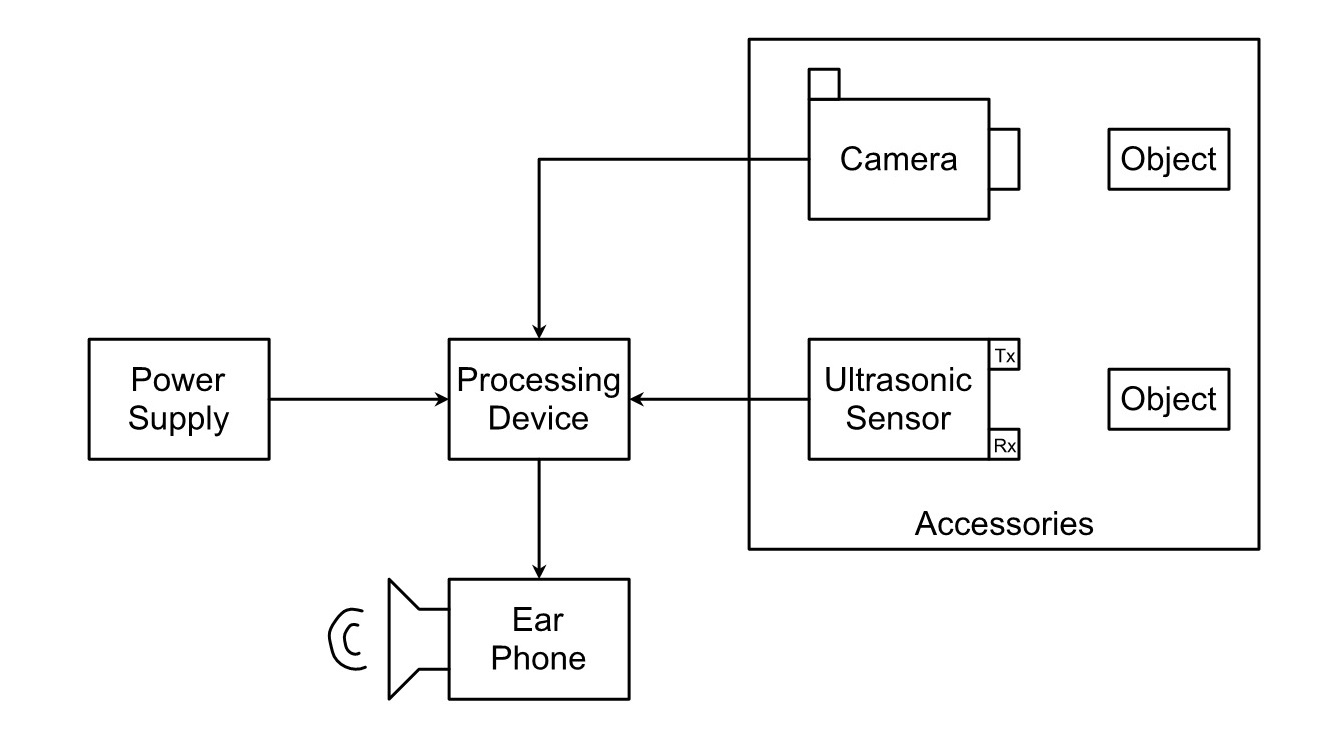
\includegraphics[width=325px]{block_1.jpeg}
	\captionof{figure}{Block Diagram}
\end{frame}
%----------------------------------------------------------------------------------------
\section{BLOCK DIAGRAM DESCRIPTION}
\begin{frame}
	\frametitle{BLOCK DIAGRAM DESCRIPTION}
	The block diagram consists of camera unit, sensor unit, processing unit, power and output unit.
		\begin{itemize}
		\item The \textbf{Camera Unit} is responsible for capturing objects while the sensor unit provides the distance of object from unit.
		\item The \textbf{Processing Unit} plays an important role in detecting and identifying objects (image processing) ,it also receives data from ultrasonic sensor then instruct the user about object identified and distance it is located at (So the user can navigate accordingly).
		\item The \textbf{Output Unit} provides output to user in terms of audio signal using ear phones.
	    \end{itemize}
\end{frame}
%----------------------------------------------------------------------------------------

%\section{PLANNING} % Sections are added in order to organize your presentation into discrete blocks, all sections and subsections are automatically output to the table of contents as an overview of the talk but NOT output in the presentation as separate slides

%------------------------------------------------

%\subsection{Paragraphs and Lists}
%\section{PLANNING}
%\begin{frame}
%	\frametitle{PLANNING}
%		\begin{itemize}
%		\item The aim is to create a Good user interface to a blind person.
%		\item First, we identify actual problems they faced in their daily life.
%		\item Study and Research on Multiple papers and projects.
%		\item Solve that problem by using two accessories.
%		\begin{itemize}
%			\item Smart Glasses - for capturing and identifying images in front of them and output goes to earphones.
%			\item Smart Shoes - For improvement action of Walk and its output goes to Vibrating Sensor.
%	    \end{itemize}
%   	\item We collect multiple resources to make it affordable and sustainable.
%    	\item Now, Working on its Simulation part.
%    	\item Once Done, We will move to make its actual Model.
%	\end{itemize}
%\end{frame}
%------------------------------------------------
\section{FLOWCHART}
\begin{frame}
	\frametitle{FLOWCHART}
	\centering
	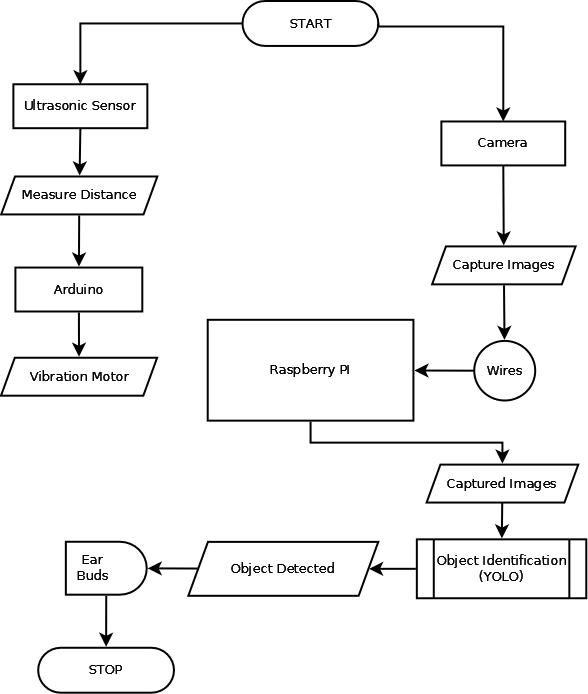
\includegraphics[width=160px]{Diagram1.png}
	\captionof{figure}{Flowchart}
\end{frame}
%------------------------------------------------
\section{WORKING}
\begin{frame}
	\frametitle{WORKING}
	\begin{enumerate}
	\item The Raspberry PI camera start capturing the frames, after the command is being issued by Raspberry PI.
	\item The Raspberry PI will process this captured frames to identify and detect objects using YOLO algorithm.
	\item At the same time, Along with identification and detection of objects it will also measure its distance. 
	\item The object with less distance will be given priority for further processing.
	\item Simultaneously, Ultrasonic sensor along with Arduino UNO will calculate distance and notify user about closer objects with the help of vibration motor.
	\item The objects detected by YOLO algorithm will be made available to the user in form of audio signal through ear buds.
	\end{enumerate}
\end{frame}
%------------------------------------------------
%\section{CODE FOR OBJECT DETECTION AND IDENTIFICATION}
%\begin{frame}
%	\frametitle{CODE FOR OBJECT DETECTION AND IDENTIFICATION}
%	\begin{center}
%	\begin{minipage}{0.30\textwidth}
%		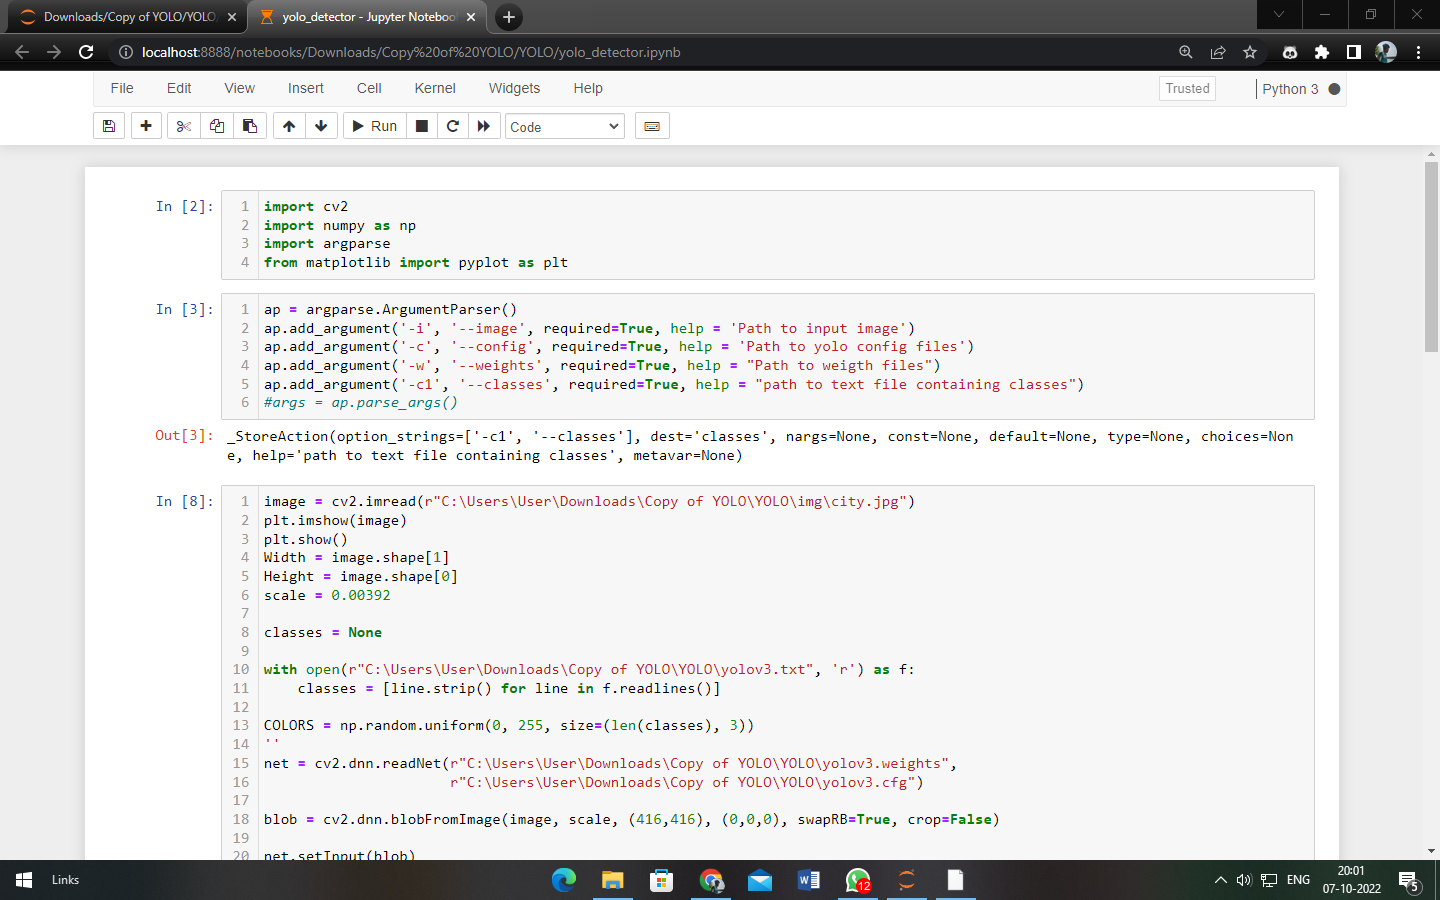
\includegraphics[width=\textwidth]{Screenshot (3).png}
%		\captionof{figure}{Code Part 1}
%	\end{minipage}\hfill
%	\begin{minipage}{0.30\textwidth}
%	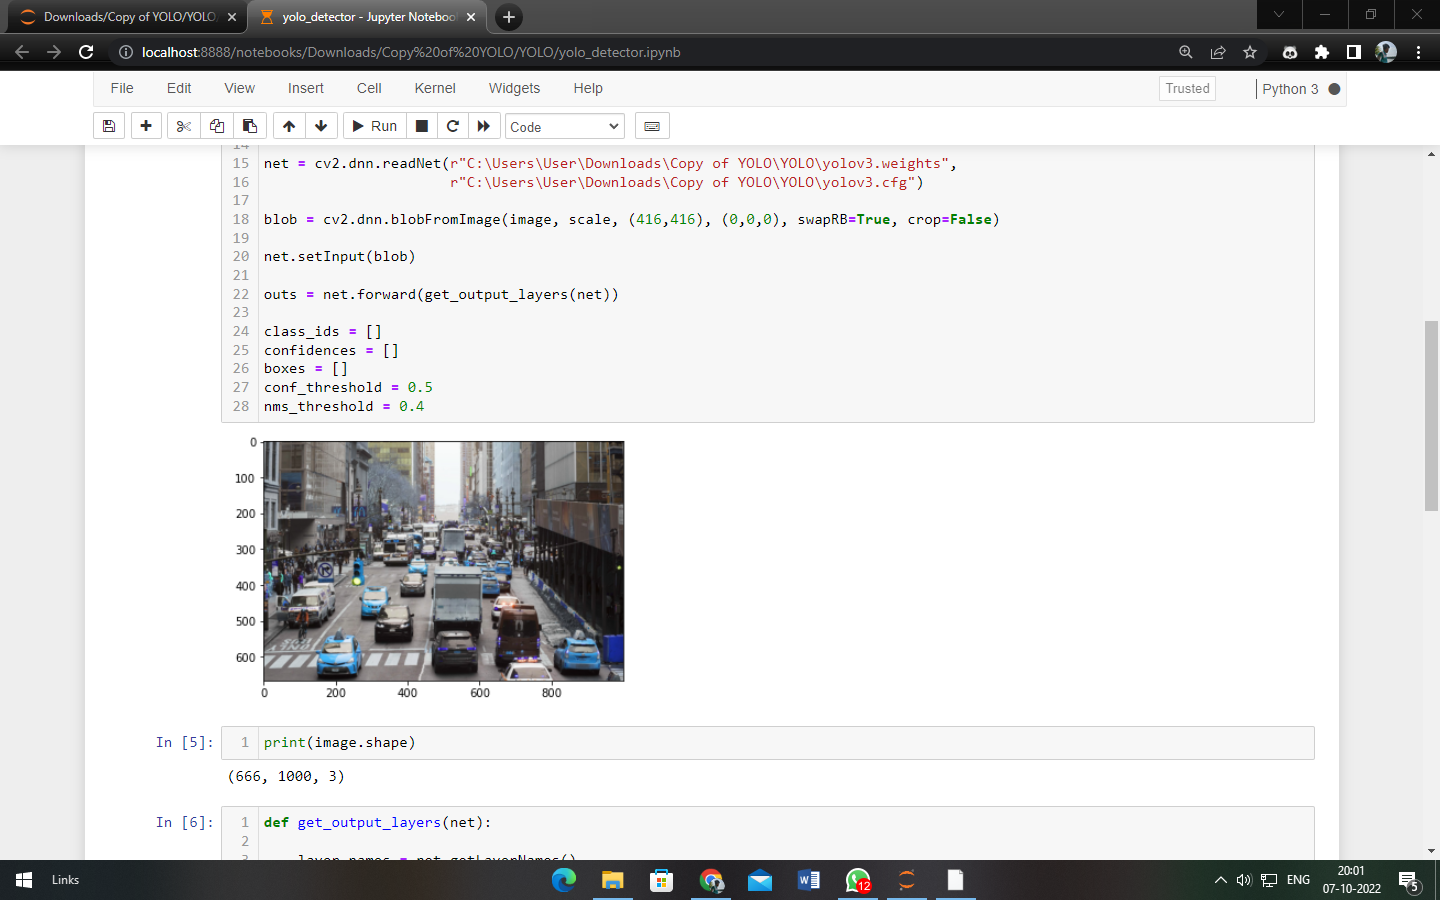
\includegraphics[width=\textwidth]{Screenshot (4).png}
%	\captionof{figure}{Code Part 2}
%\end{minipage}\hfill
%	\begin{minipage}{0.30\textwidth}
%	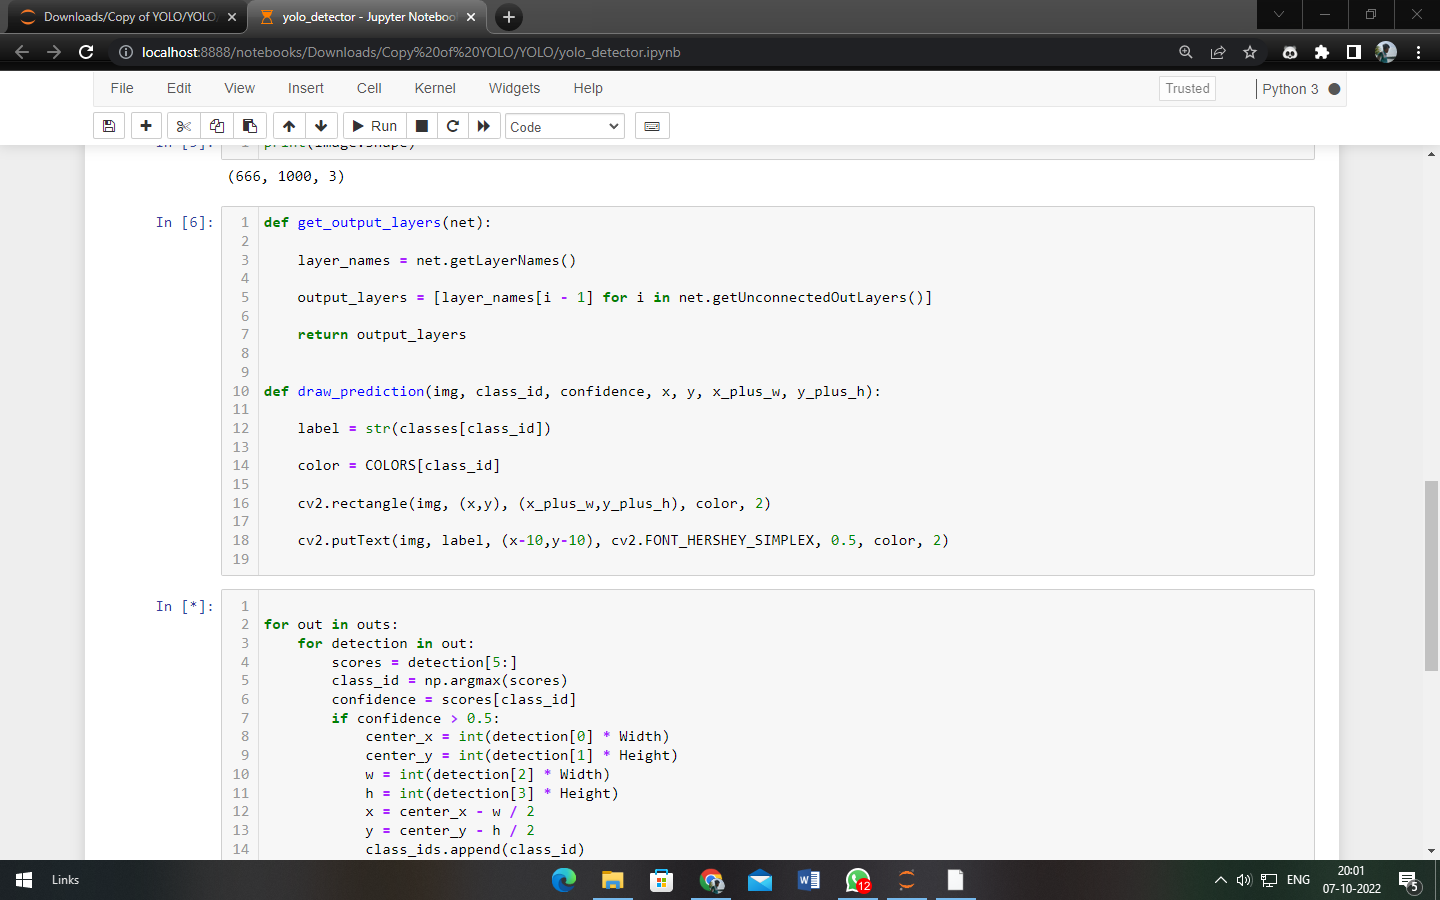
\includegraphics[width=\textwidth]{Screenshot (5).png}
%	\captionof{figure}{Code Part 3}
%\end{minipage}\hfill
%\centering
%	\begin{minipage}{0.30\textwidth}
%	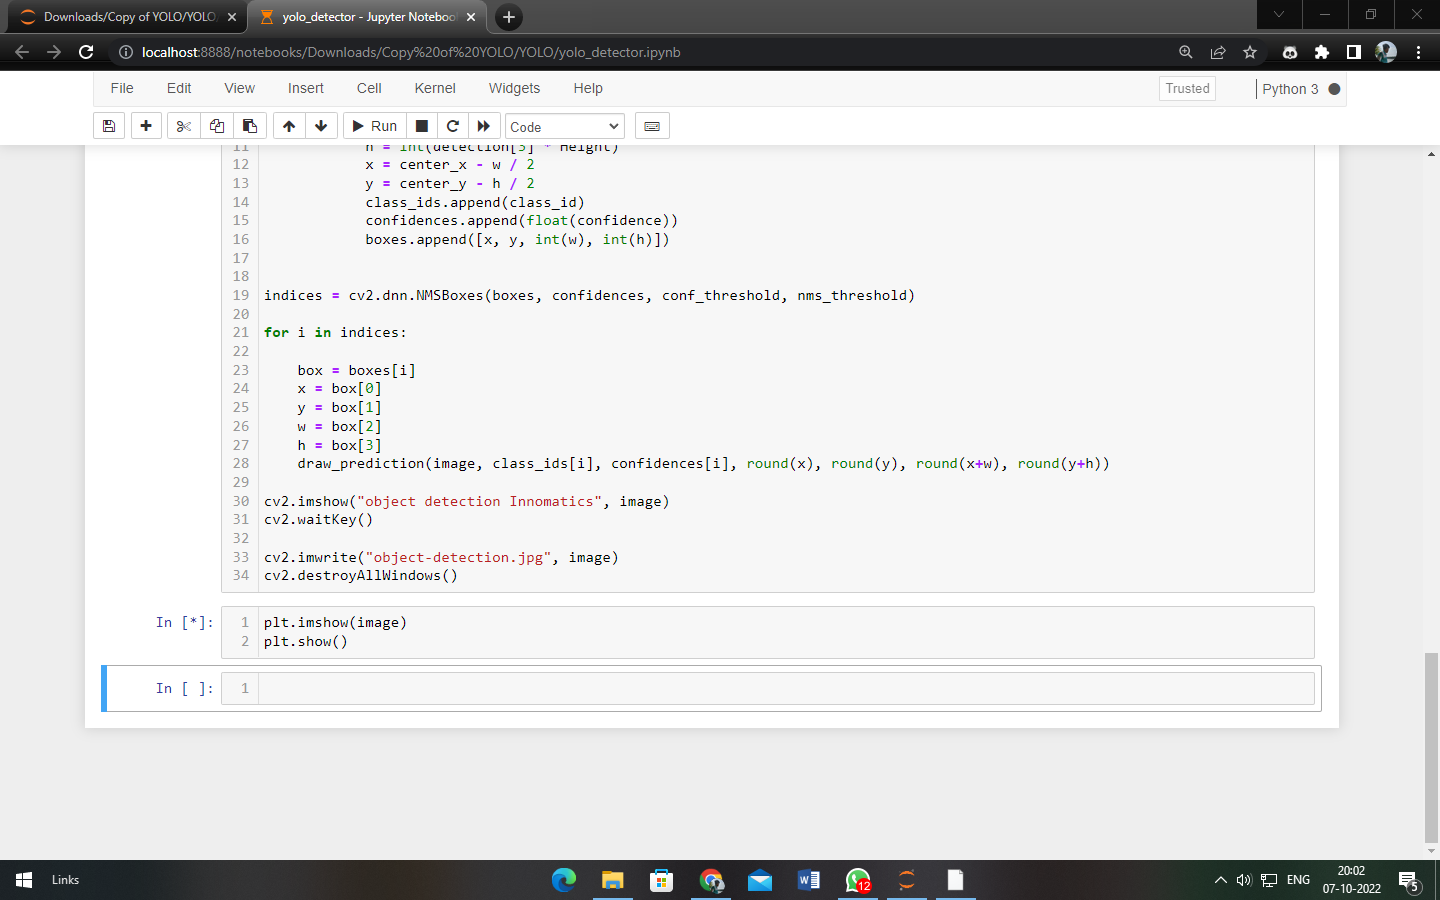
\includegraphics[width=\textwidth]{Screenshot (6).png}
%	\captionof{figure}{Code Part 4}
%\end{minipage}
%\end{center}
%\end{frame}
%------------------------------------------------
\section{CODE}
\begin{frame}
	\frametitle{CODE}
	\centering
	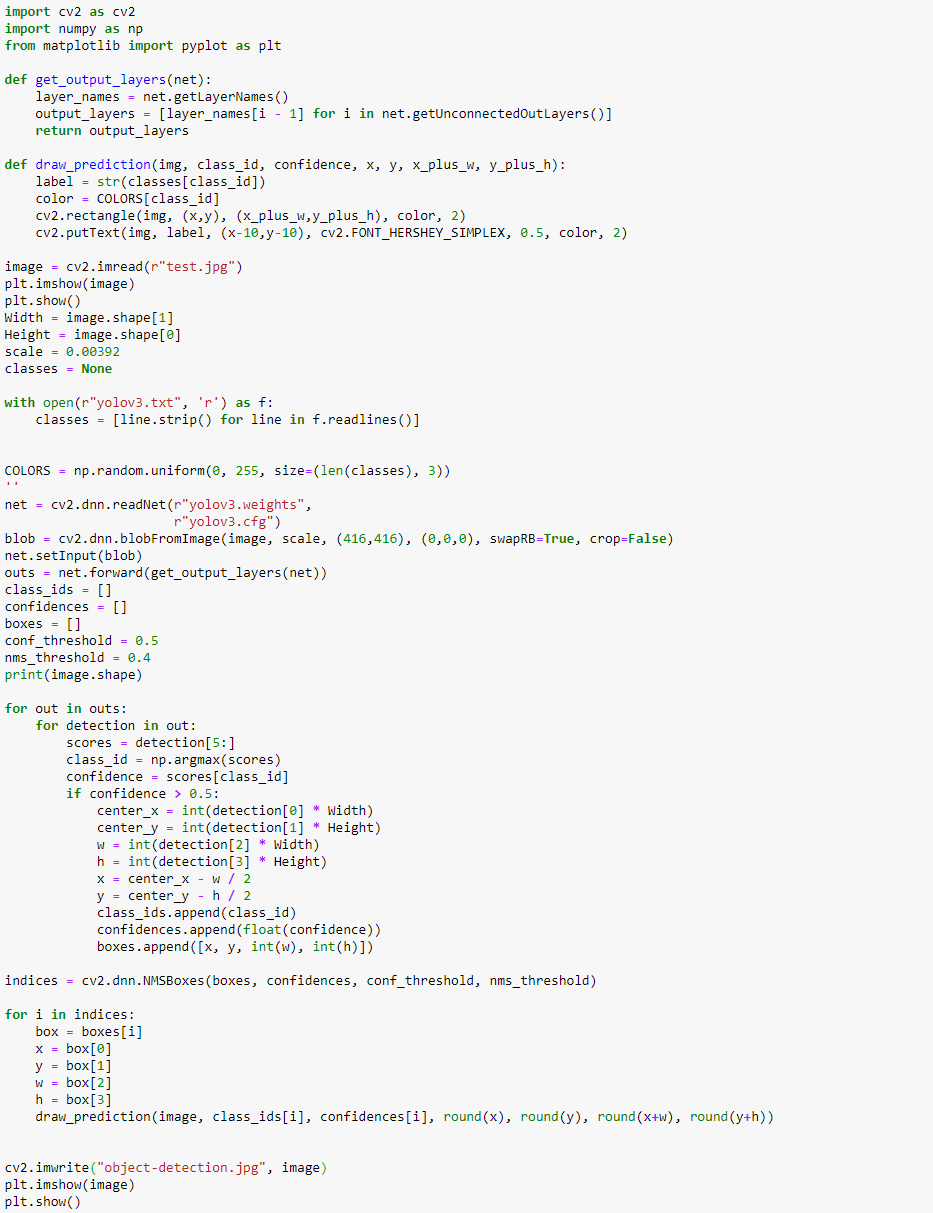
\includegraphics[height=180px, width=200px]{code.png}
	\captionof{figure}{Code for object detection and identification}
\end{frame}

\begin{frame}
	\frametitle{CODE}
	\centering
	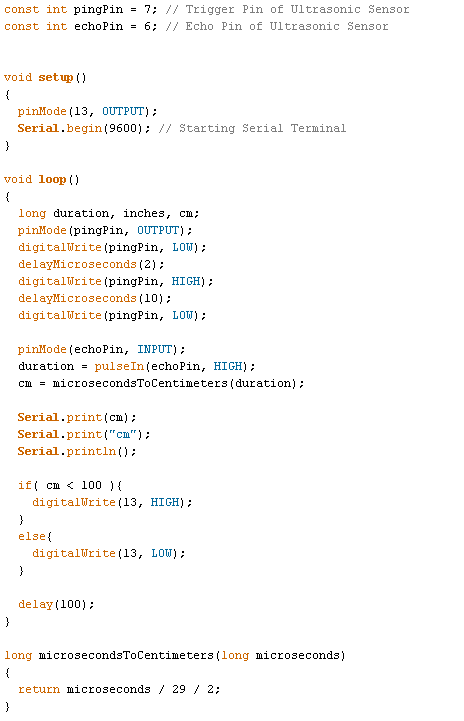
\includegraphics[height=180px, width=200px]{code_ard.png}
	\captionof{figure}{Code for Arduino}
\end{frame}
%------------------------------------------------
\section{OUTPUT}
\begin{frame}
	\frametitle{OUTPUT}
	\bigskip  
		\begin{center}
		\begin{minipage}{0.45\textwidth}
			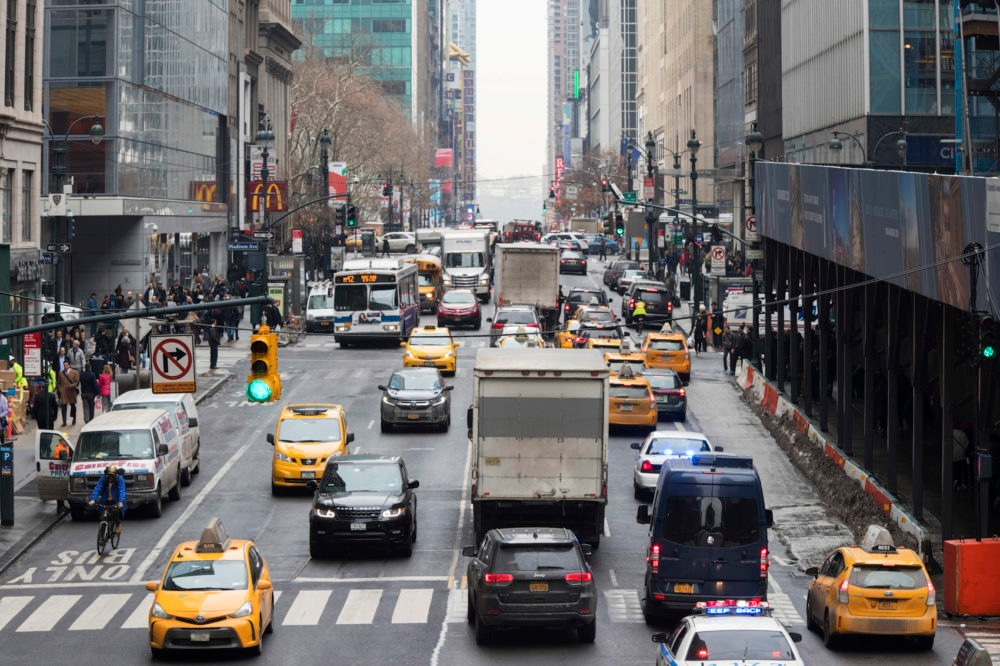
\includegraphics[height=150px,width=\textwidth]{before.jpeg}
			\captionof{figure}{Before}
		\end{minipage} \hspace{0.5cm}
		\begin{minipage}{0.45\textwidth}
			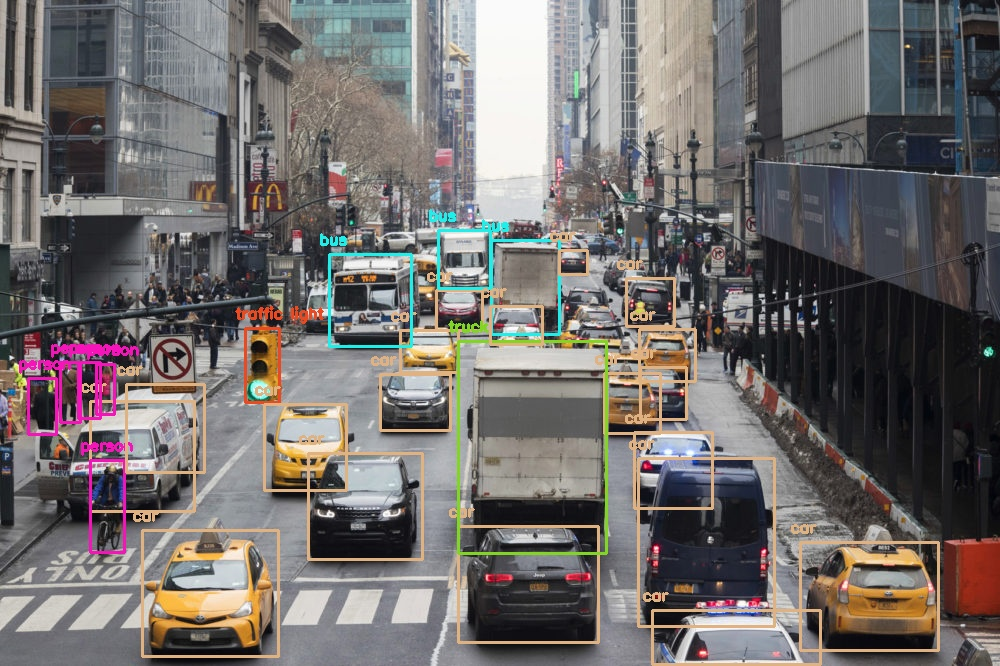
\includegraphics[height=150px,width=\textwidth]{after.jpeg}
			\captionof{figure}{After} 
		\end{minipage}
		\label{name_label}
	\end{center}
\end{frame}
\begin{frame}
	\frametitle{OUTPUT}
	\bigskip  
		\begin{center}
		\begin{minipage}{0.45\textwidth}
			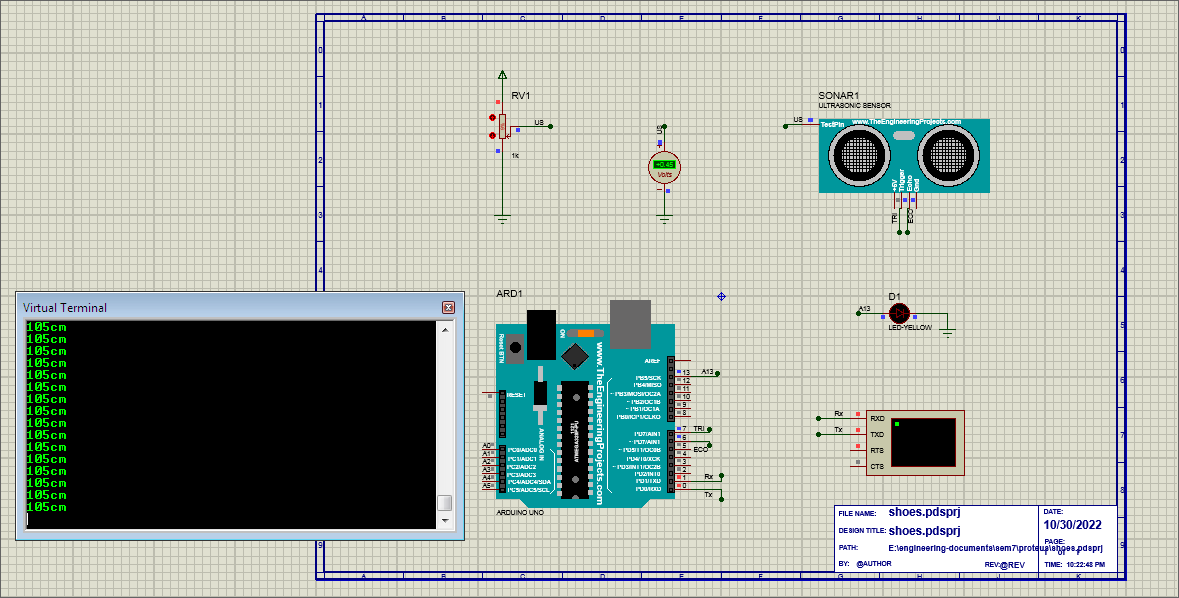
\includegraphics[height=150px,width=\textwidth]{beforeA.png}
			\captionof{figure}{Before}
		\end{minipage} \hspace{0.5cm}
		\begin{minipage}{0.45\textwidth}
			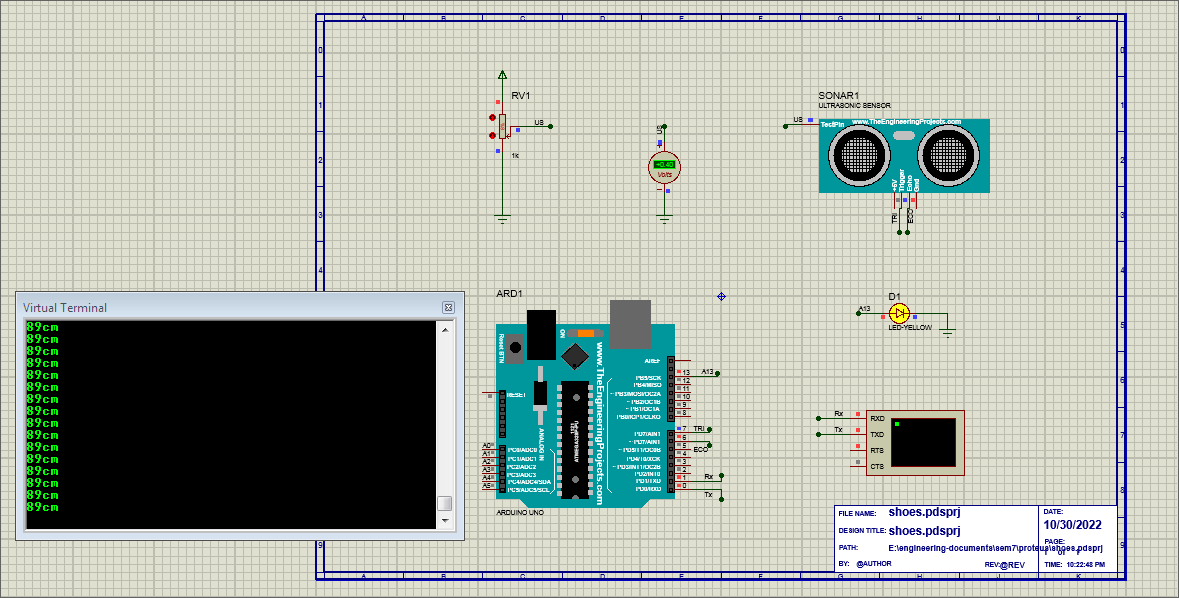
\includegraphics[height=150px,width=\textwidth]{afterA.png}
			\captionof{figure}{After} 
		\end{minipage}
		\label{name_label}
	\end{center}
\end{frame}
%------------------------------------------------

%\section{PARTIAL EXPLAINATION}
%\begin{frame}
%	\frametitle{PARTIAL EXPLAINATION}
%	%\framesubtitle{Bullet Points and Numbered Lists} % Optional subtitle
%	\begin{itemize}
%\item The glasses will detect the object which is in front of the person.
%\item With the help of a camera model, we capture the image and process it in raspberry Pi with the help %of the yolo model.
%\item The shoes will detect the object that is in front of the foot.
%\item With the help of ultrasonic sensors, we detect the object and process the input in ESP -32 and send %the output to the vibrating motor.
%	\end{itemize}
%\end{frame}
%------------------------------------------------
\section{COMPONENTS}
\begin{frame}
	\frametitle{COMPONENTS}
	%\framesubtitle{Bullet Points and Numbered Lists} % Optional subtitle
	
	\begin{center}
		\begin{minipage}{0.30\textwidth}
			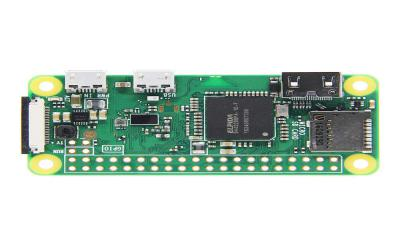
\includegraphics[width=\textwidth]{./resized_400x250/Raspberry_zero.jpg}
			\captionof{figure}{Raspberry PI Zero}
		\end{minipage}\hfill
		\begin{minipage}{0.30\textwidth}
			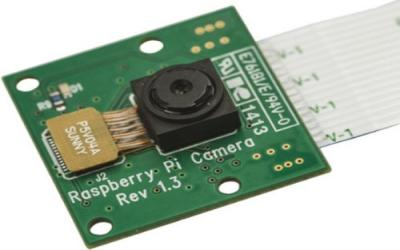
\includegraphics[width=\textwidth]{./resized_400x250/raspberry pi cam.jpg}
\captionof{figure}{Raspberry PI CAM} 
		\end{minipage}\hfill
		\begin{minipage}{0.30\textwidth}
			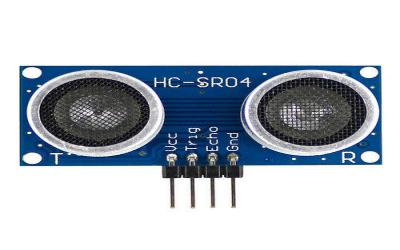
\includegraphics[width=\textwidth]{./resized_400x250/ultrasonic sensor.jpg}
\captionof{figure}{Ultrasonic Sensor} 
		\end{minipage}
	
			\begin{minipage}{0.30\textwidth}
		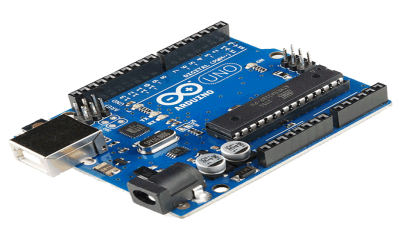
\includegraphics[width=\textwidth]{./resized_400x250/arduino.png}
		\captionof{figure}{Arduino UNO}
	\end{minipage}\hfill
	\begin{minipage}{0.30\textwidth}
		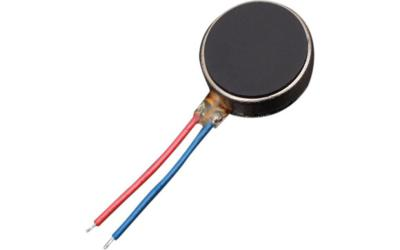
\includegraphics[width=\textwidth]{./resized_400x250/vibrating motor.jpg}
		\captionof{figure}{Vibrating Motor}
	\end{minipage}\hfill
	\begin{minipage}{0.30\textwidth}
		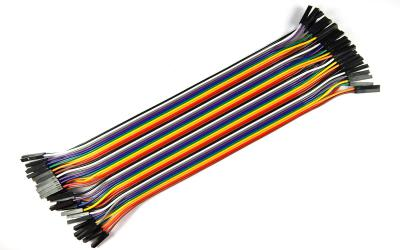
\includegraphics[width=\textwidth]{./resized_400x250/wire.jpg}
		\captionof{figure}{Wires}  
	\end{minipage}
		%\captionof{figure}{Total caption }
		%\label{name_label}
	\end{center}
	
\end{frame}

\begin{frame}
	\frametitle{COMPONENTS}
	%\framesubtitle{Bullet Points and Numbered Lists} % Optional subtitle
	
	\begin{center}	
		\begin{minipage}{0.30\textwidth}
			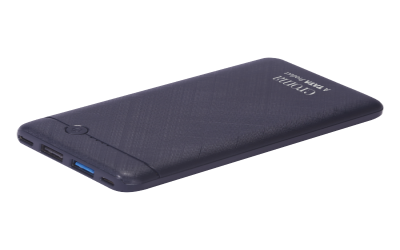
\includegraphics[width=\textwidth]{chromo.png}
			\captionof{figure}{Battery}
		\end{minipage}\hspace{1cm}
		\begin{minipage}{0.30\textwidth}
			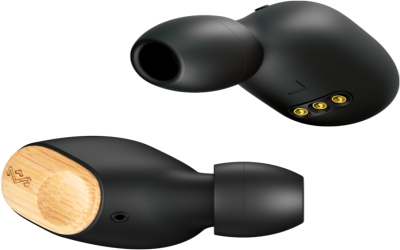
\includegraphics[width=\textwidth]{ear.png}
			\captionof{figure}{Ear Buds}
		\end{minipage}
		%\captionof{figure}{Total caption }
		%\label{name_label}
	\end{center}
\end{frame}

%------------------------------------------------
\section{ADVANTAGES AND APPLICATIONS}
\begin{frame}
	\frametitle{ADVANTAGES AND APPLICATIONS}
	\textbf{ADVANTAGES}
	\begin{enumerate}
	\item Both indoor and outdoor navigation are possible with the device.
	\item Detects obstacles and notifies the blind person through vibration and speech production.
	\item The devices placed are comfortable and easy to handle. 
	\end{enumerate}
 \vspace{1.5cm}
	\textbf{APPLICATIONS}
	\begin{enumerate}
	\item It can be used for providing a set of useful features :- light detection, color detection, object recognition, and banknote recognition
	\end{enumerate}
\end{frame}
%------------------------------------------------

%\begin{frame}
%	\frametitle{COSTING}
%	%\framesubtitle{Bullet Points and Numbered Lists} % Optional subtitle
%	\begin{table}
%		\large
%		\begin{tabular}{l l l l}
%			\toprule
%			\textbf{SR No.} & \textbf{Component} & \textbf{Nos} & \textbf{Cost}\\
%			\midrule
%			1 & Raspberry PI Zero & 1 & 5000 \\
%			2 & Raspberry PI CAM & 1 & 400 \\
%			3 & Ultrasonic Sensor & 2 & 60 \\
%			4 & ESP32 Module & 2 & 540 \\
%			5 & Vibration Motor & 2 & 30 \\
%			6 & Power Bank & 1 & 500 \\
%			7 & Ear Buds & 1 & 800 \\
%			8 & Wires & - & 50 \\
%			 & Approx. & & 8000 \\
%			\bottomrule
%		\end{tabular}
%		\caption{Costing}
%	\end{table}
%\end{frame}

%------------------------------------------------
\section{CONCLUSION}
\begin{frame}
	\frametitle{CONCLUSION}
	Visually impaired people faced many problems in their daily life, and while traveling they always depend on any person or guide dog. Blind Stick is very helpful for them but Stick has certain restrictions. We created a navigation device for visually impaired people so that they can perform their daily tasks.
	
	\bigskip
	
	There are certain Devices already available in the market but they cannot solve the actual problem. Our project is an integrated system of those devices.
	
\bigskip

In this paper, We present wearable Accessories in the form of Smart Glasses and Smart Shoes for visually impaired people to deal with their Tasks. Smart Glasses Capture images in front of those objects and recognize them and convert it into an audio form which is then sent to the earphones.
\end{frame}
%------------------------------------------------
\begin{frame}
	\frametitle{REFERENCES}
\begin{enumerate}
	\item Nishajith.A, Nivedha.J, Shilpa.S.Nair \& Prof. Mohammed Shaffi.J, “SMART CAP – WEARABLE VISUAL GUIDANCE SYSTEM FOR BLIND”, ISBN:978-1-5386-2456-2.
\item Arjun Pardasani, Prithviraj N Indi, Sashwata Banerjee, Aditya Kamal \& Vaibhav Garg, “Smart Assistive Navigation Devices for Visually Impaired People”, ISBN:978-1-7281-1322-7.
\item Joe Louis Paul I, Sasirekha S, Mohanavalli S, Jayashree C, Moohana Priya P \& Monika K, “Smart Eye for Visually Impaired-An aid to help the blind people”, ISBN:978-1-5386-9471-8.
\item N.Loganathan, K.Lakshmi, N.Chandrasekaran, S.R.Cibisakaravarthi, R.Hari Priyanga \& K.HarshaVarthini, “Smart Stick For Blind People”, ISBN:978-1-7281-5197-7.
	\end{enumerate}
\end{frame}
%----------------------------------------------------------------------------------------
%	CLOSING SLIDE
%----------------------------------------------------------------------------------------

\begin{frame}[plain] % The optional argument 'plain' hides the headline and footline
	\begin{center}
\vspace{3cm}
		{\Huge THANK YOU}
	\end{center}
\end{frame}

%----------------------------------------------------------------------------------------

\end{document} 
